% Drawing 69/05-1 -- folder 69, batch 05, archive page 81 (PDF page 82).
% Transcription: Un fragment de graphe cubique à faces pentagonales (six pentagones autour d'un pentagone central, à la manière d'un dodécaèdre déplié). Les arêtes portent les numéros 1 à 5 ; les trois arêtes numérotées 3 qui forment un couplage sont repassées en gras. Les sommets sont marqués : au pentagone central, $\xi_{12}$, $\xi_{45}$, $\xi_{23}$, $\xi_{51}$, $\xi_{34}$ ; à l'extérieur, $\xi_{35}$, $\xi_{4,12}$ \uncertain{}, $\xi_{13}$, $\xi_{25}$, $\xi_{41}$, $\xi_{5,3}$, $\xi_{2,4}$, $\xi_{3,1}$, $\xi_{52}$, $\xi_{14}$. En haut à gauche, un petit pentagone raturé, une de ses arêtes en gras.
% Kind: fragment of a cubic graph with pentagonal faces (half dodecahedron). Method 3 (encoded, rendered from the data). Status: ok.
% Notes: A central pentagon xi_12, xi_45, xi_23, xi_51, xi_34 surrounded by five pentagons: half a dodecahedron, 15 vertices, 20 edges, 6 pentagonal faces (the transcription says "six pentagones autour d'un pentagone central"; it is five around the central one, six in all). The edges carry the numbers 1 to 5 (an edge colouring read from the page, kept in the .json); the three thick edges numbered 3 (xi_12 xi_45, xi_25 xi_41, xi_51 xi_2,4) form a matching; a fourth edge marked 3 (xi_52 xi_14) is not thick. Vertex labels as the transcription reads them (xi_4,12 uncertain; the page has xi_51 for the vertex below the central pentagon). The small struck pentagon at the top left is drawn grey.
% Coordinates: 1 unit = 1 mm = 1/100 of the crop width (bbox in page fractions: [0.18, 0.06, 0.68, 0.33]).
% Redrawn by Claude (claude-opus-5-5), issue #73, 2026-11-07; not checked by a human; not compiled (no TeX in the session).
% Rights: reproduces part of the work -- behind RENDER_TRANSCRIPTS, never published by itself.
\documentclass[tikz,border=3pt]{standalone}
\usepackage{amsmath,amssymb}
\usetikzlibrary{patterns,arrows.meta}
\tikzset{pencil/.style={black!45}, struck/.style={black!35}, mark/.style={circle,draw,inner sep=1.3pt}, pt/.style={circle,fill,inner sep=0.9pt}, opt/.style={circle,draw,fill=white,inner sep=1.1pt}}
\begin{document}
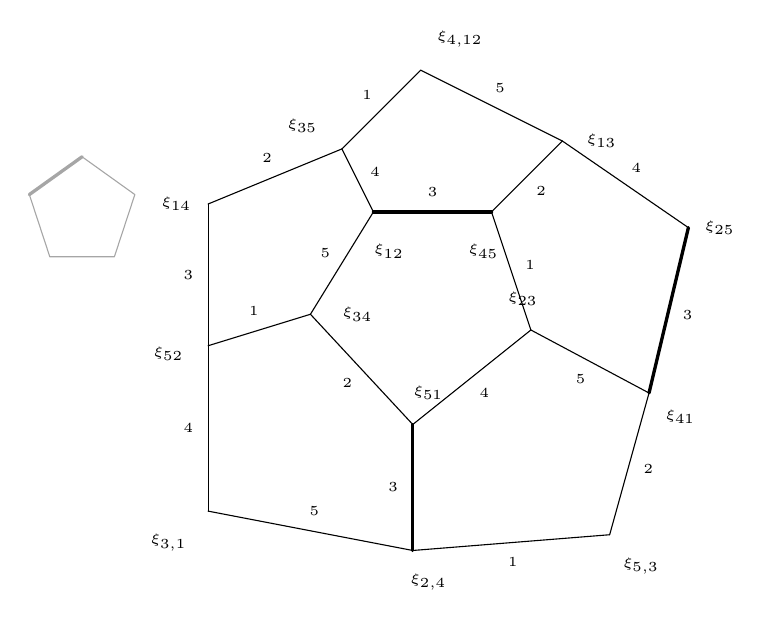
\begin{tikzpicture}[x=1mm,y=1mm,line cap=round,line join=round,font=\scriptsize]
\draw[very thick] (55,-29) -- (70,-29);
\draw (70,-29) -- (75,-44);
\draw (75,-44) -- (60,-56);
\draw (60,-56) -- (47,-42);
\draw (47,-42) -- (55,-29);
\draw (34,-28) -- (51,-21);
\draw (51,-21) -- (55,-29);
\draw (51,-21) -- (61,-11);
\draw (61,-11) -- (79,-20);
\draw (79,-20) -- (70,-29);
\draw (79,-20) -- (95,-31);
\draw[very thick] (95,-31) -- (90,-52);
\draw (90,-52) -- (75,-44);
\draw (90,-52) -- (85,-70);
\draw (85,-70) -- (60,-72);
\draw[very thick] (60,-72) -- (60,-56);
\draw (34,-67) -- (60,-72);
\draw (34,-67) -- (34,-46);
\draw (34,-46) -- (47,-42);
\draw (34,-46) -- (34,-28);
\node[inner sep=1pt] at (62.5,-26.5) {\tiny $3$};
\node[inner sep=1pt] at (74.9,-35.7) {\tiny $1$};
\node[inner sep=1pt] at (69.1,-52) {\tiny $4$};
\node[inner sep=1pt] at (51.7,-50.7) {\tiny $2$};
\node[inner sep=1pt] at (48.9,-34.2) {\tiny $5$};
\node[inner sep=1pt] at (41.5,-22.2) {\tiny $2$};
\node[inner sep=1pt] at (55.2,-23.9) {\tiny $4$};
\node[inner sep=1pt] at (54.2,-14.2) {\tiny $1$};
\node[inner sep=1pt] at (71.1,-13.3) {\tiny $5$};
\node[inner sep=1pt] at (76.3,-26.3) {\tiny $2$};
\node[inner sep=1pt] at (88.4,-23.4) {\tiny $4$};
\node[inner sep=1pt] at (94.9,-42.1) {\tiny $3$};
\node[inner sep=1pt] at (81.3,-50.2) {\tiny $5$};
\node[inner sep=1pt] at (89.9,-61.7) {\tiny $2$};
\node[inner sep=1pt] at (72.7,-73.5) {\tiny $1$};
\node[inner sep=1pt] at (57.5,-64) {\tiny $3$};
\node[inner sep=1pt] at (47.5,-67) {\tiny $5$};
\node[inner sep=1pt] at (31.5,-56.5) {\tiny $4$};
\node[inner sep=1pt] at (39.8,-41.6) {\tiny $1$};
\node[inner sep=1pt] at (31.5,-37) {\tiny $3$};
\node[inner sep=1pt] at (57,-34) {\tiny $\xi_{12}$};
\node[inner sep=1pt] at (69,-34) {\tiny $\xi_{45}$};
\node[inner sep=1pt] at (74,-40) {\tiny $\xi_{23}$};
\node[inner sep=1pt] at (62,-52) {\tiny $\xi_{51}$};
\node[inner sep=1pt] at (53,-42) {\tiny $\xi_{34}$};
\node[inner sep=1pt] at (46,-18) {\tiny $\xi_{35}$};
\node[inner sep=1pt] at (66,-7) {\tiny $\xi_{4,12}$};
\node[inner sep=1pt] at (84,-20) {\tiny $\xi_{13}$};
\node[inner sep=1pt] at (99,-31) {\tiny $\xi_{25}$};
\node[inner sep=1pt] at (94,-55) {\tiny $\xi_{41}$};
\node[inner sep=1pt] at (89,-74) {\tiny $\xi_{5,3}$};
\node[inner sep=1pt] at (62,-76) {\tiny $\xi_{2,4}$};
\node[inner sep=1pt] at (29,-71) {\tiny $\xi_{3,1}$};
\node[inner sep=1pt] at (29,-47) {\tiny $\xi_{52}$};
\node[inner sep=1pt] at (30,-28) {\tiny $\xi_{14}$};
\draw[struck] (18,-22) -- (11.3,-26.8) -- (13.9,-34.7) -- (22.1,-34.7) -- (24.7,-26.8) -- cycle;
\draw[very thick,struck] (18,-22) -- (11.3,-26.8);
\end{tikzpicture}
\end{document}
